\section{The two priority signals}
\label{sec:primary}

\subsection{TIC 80387959: successful prediction tests with an unresolved host}

TIC 80387959 provides the clearest successful prediction test in this
investigation. Its adopted clock has period $P=4.192168718052227$ d,
reference midpoint $t_0=1575.375831123655$ BTJD, and fixed box duration
$D=0.092736$ d ($2.225664$ h). Throughout this paper,
$\mathrm{BTJD}=\mathrm{BJD}_{\mathrm{TDB}}-2457000$.
The digits specify the saved prediction; they do not imply that the physical
orbit is known to the displayed precision. Predictions based on the earlier
sectors were frozen before retrieval of QLP sectors 90 and 100. Without
adjusting the clock, the original follow-up procedure measured depths of
$621\pm98$ and $651\pm114$ ppm, respectively (Figure~\ref{fig:803holdout}).
Five and three events entered those measurements, of which four and two
passed the procedure's individual support criterion. The propagated timing
spreads, 0.02477 and 0.02679 d, were below the half-duration gate of
0.046368 d. These results support recurrence at the earlier prediction,
while leaving the variable source and physical explanation undetermined.

\begin{figure}[tbp]
\centering
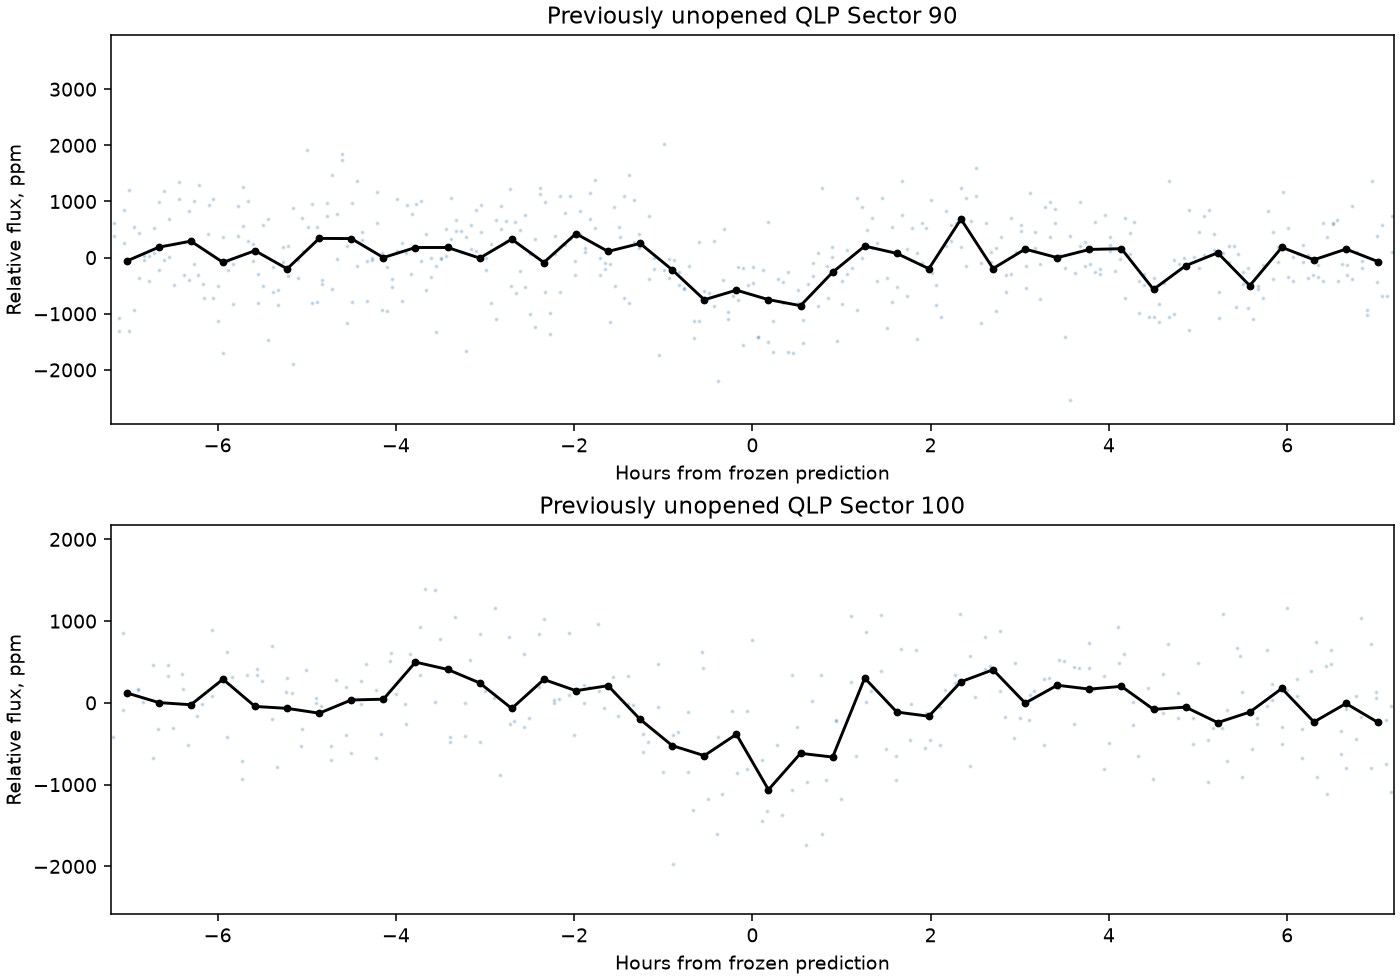
\includegraphics[width=0.96\linewidth]{figures/803-holdout.png}
\caption{TIC 80387959 in QLP sectors 90 and 100 at the prediction fixed
before those products were retrieved. These are the original follow-up
reductions, with their original preprocessing and sampling. Positive
recurrence at the fixed clock is evidence about the signal; it does not
identify the star producing it. Displayed measurement errors are
conditional on the adopted processing and noise model.}
\label{fig:803holdout}
\end{figure}

A subsequent retrospective test used native corrected flux from all six
already inspected sectors, without an additional global flattening filter.
It fitted an exposure-integrated box simultaneously with separate local
intercepts and slopes for each event. Table~\ref{tab:803depths} reports these
measurements, which have different samples and nuisance models from the
original prediction test. All six sectors and every single-event omission
retain a positive depth; the smallest omitted-event depth is 494 ppm in
sector 100. Thirty event windows enter this particular analysis.
Neither these windows nor alternative reductions of their exposures are
thirty independent confirmations of a planetary interpretation.

\begin{table}[tbp]
\centering
\caption{TIC 80387959: retrospective joint local-baseline box fits.
The final column applies a heuristic time-averaging noise inflation to the
same depth estimates. All errors are conditional, not complete uncertainty
budgets or calibrated search significances.}
\label{tab:803depths}
\begin{tabular}{rlrrr}
\toprule
Sector & Product & Events & Depth (ppm) & Adjusted error (ppm) \\
\midrule
10  & TESS-SPOC PDCSAP & 4 & $1038\pm109$ & 113 \\
36  & TESS-SPOC PDCSAP & 6 & $813\pm87$   & 92 \\
37  & TESS-SPOC PDCSAP & 5 & $904\pm91$   & 105 \\
63  & TESS-SPOC PDCSAP & 5 & $807\pm93$   & 130 \\
90  & QLP DET\_FLUX   & 6 & $613\pm89$   & 92 \\
100 & QLP DET\_FLUX   & 4 & $582\pm99$   & 133 \\
\bottomrule
\end{tabular}
\end{table}

\begin{figure}[tbp]
\centering
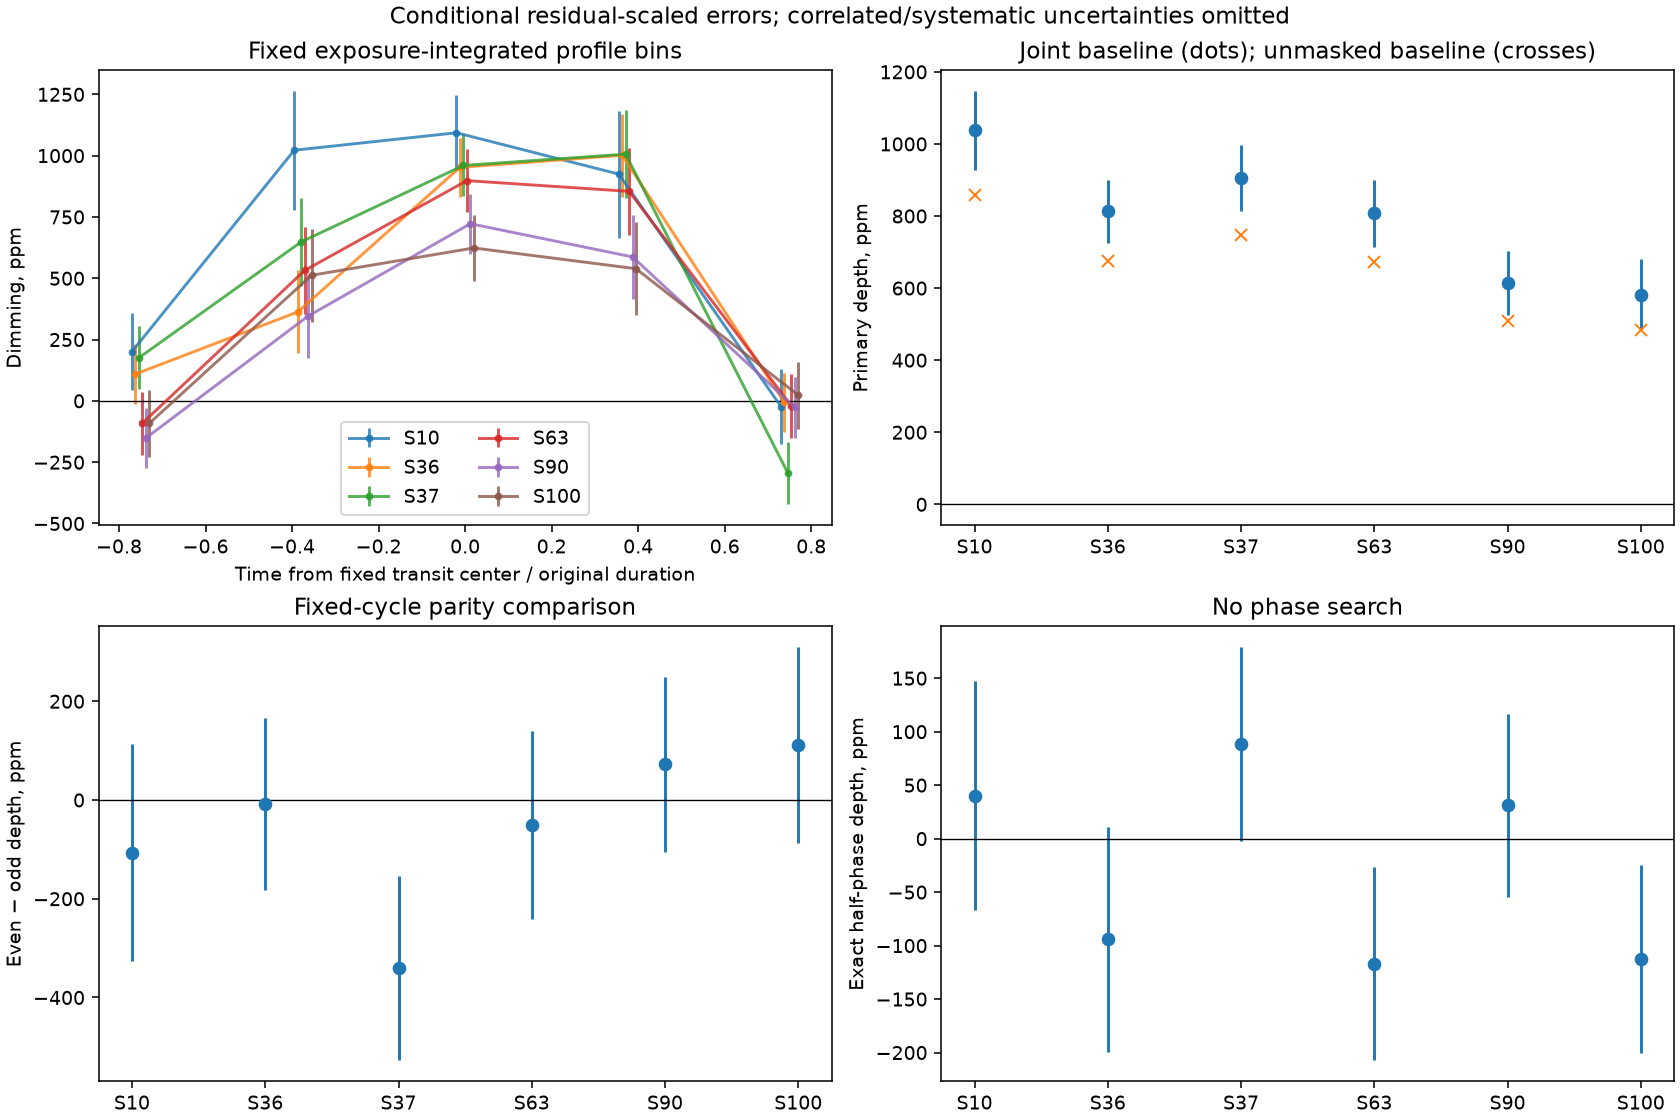
\includegraphics[width=0.97\linewidth]{figures/803-shape.png}
\caption{Six-sector fixed-clock shape, depth, parity, and half-phase tests
for TIC 80387959. Native corrected-flux models jointly fit local event
baselines, without additional global flattening. All data were already
inspected before this retrospective analysis. Conditional errors omit a
complete correlated-noise and dilution model. A positive dip across these
tests does not exclude a blended stellar eclipse.}
\label{fig:803shape}
\end{figure}

No coherent odd/even difference or secondary eclipse exactly half a cycle
away emerges (Figure~\ref{fig:803shape}). An isolated sector-36
ingress-minus-egress contrast of $-639\pm233$ ppm is retained rather than
interpreted as a replicated asymmetry. A secondary at another phase,
strong dilution, or an unresolved companion could evade these checks.
The descriptive depth means differ between the four older TESS-SPOC
sectors ($877\pm47$ ppm) and the later QLP sectors ($599\pm66$ ppm).
This is not established physical depth evolution. Same-epoch paired
products give SPOC-minus-QLP differences of $+47\pm76$ ppm in sector 36
and $-163\pm96$ ppm in sector 37, offering no consistent pipeline offset.
Common-quality sampling itself changes fitted depths, and the later
QLP extraction changed beginning in sector 94 \cite{petitpas2026}.

Time-averaging diagnostics motivated by \cite{pont2006} increase the
sector-100 error from 99 to 133 ppm. Its worst event-omission depth/error
ratio is 2.96. These checks weaken the apparent precision without removing
the signal; they do not calibrate its false-alarm probability. Four-sector
orbital-harmonic tests likewise find no stable substantial modulation, but
pipeline correction can suppress broad variability and this null result
cannot exclude binaries.

Independent survey context is modestly favorable for the bright star.
One securely associated RAVE observation on 2010 May 2 gives
$5.94\pm0.87$ km s$^{-1}$, consistent with the Gaia aggregate velocity
$7.02097\pm0.32064$ km s$^{-1}$ at 1.17 combined formal error units.
Predominantly normal RAVE morphology and dwarf-like atmospheric parameters
do not constitute a companion exclusion. There is only one RAVE epoch,
the surveys have different systematics, and a faint eclipsing neighbor
would not be tested by this agreement. Gaia's available RV diagnostics
provide no strong variability flag, but no orbital sensitivity or mass
limit has been established.

\subsection{TIC 402358350: localized recurrence with a failed timing gate}

For TIC 402358350, the expanded clock frozen before sector 81 has
$P=11.769544332077816$ d, $t_0=2392.9928689397047$ BTJD, and
$D=0.144$ d ($3.456$ h). It incorporated sectors 40, 41, and 54;
sector 54 had already been examined and is not an independent test of this
expanded model. The original discovery clock was different and is retained
in the evidence record.

The primary sector-81 prediction yields $634.6\pm72.2$ ppm with two
supported events. However, its timing-profile spread of 0.09142 d exceeds
the predeclared $D/2=0.072$ d gate. Consequently this is a positive dimming
measurement with \emph{inconclusive prediction timing}, despite a formal
depth/error ratio of 8.79. The alternate expanded reduction and both
original-clock reductions also fail timing precision. All four comparisons
are shown in Figure~\ref{fig:402holdout}; selecting the deepest comparison
would not repair this failure.

\begin{figure}[tbp]
\centering
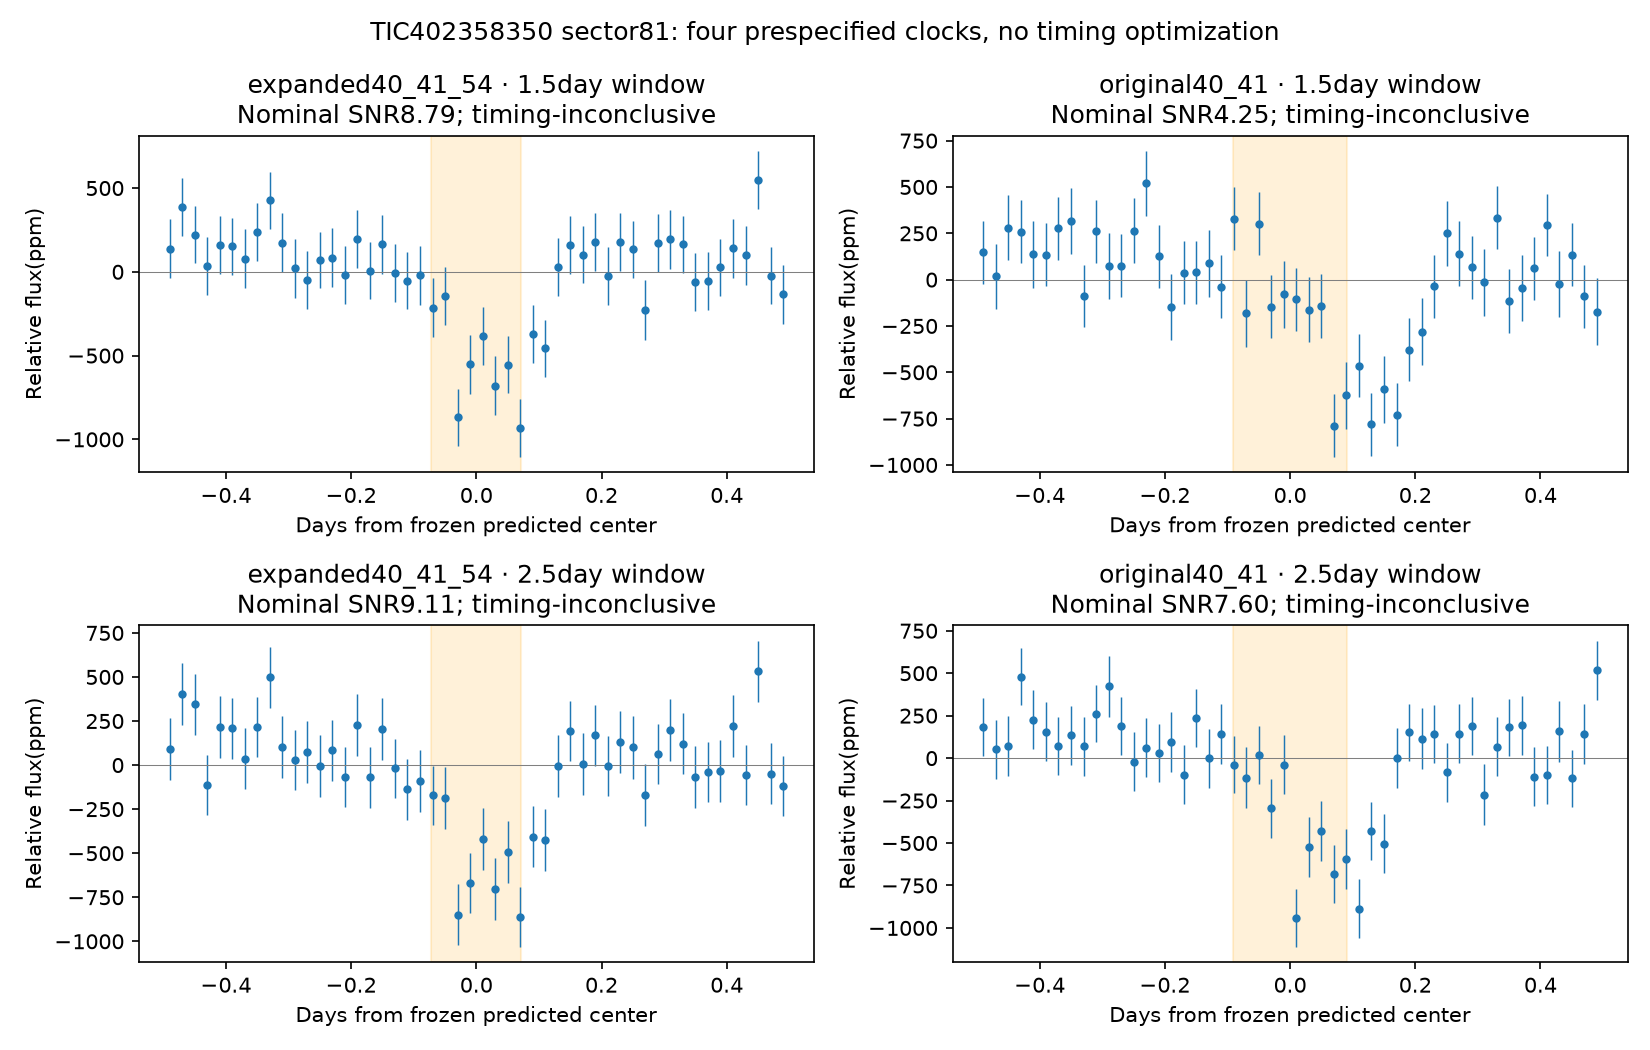
\includegraphics[width=0.96\linewidth]{figures/402-holdout.png}
\caption{Sector-81 measurements for all four predictions fixed before
access to TIC 402358350's sector-81 photometry. The expanded primary clock
places a compact dip near the predicted center, but its timing spread
exceeds the unchanged precision gate. The comparisons share the same
sector-81 photons; neither alternate preprocessing nor a positive formal
depth converts the result into a passed timing test.}
\label{fig:402holdout}
\end{figure}

A separate retrospective test directly fitted native SAP and PDCSAP
photometry, normalized by each sector's median. Polynomial baselines of
degree zero, one, and two used points outside the protected interval
$|t-t_c|\leq D$, with outer radii $3D$ or $5D$. No running-median
flattening or data-dependent clipping was added. Nine nominal centers fall
within the sector spans; one sector-40 event lies in a gap and fails
coverage for all twelve methods. The remaining eight events are positive
under every method, yielding the 590--659 ppm combined depths in
Table~\ref{tab:402baseline}. Leaving out any one event retains
569--706 ppm across the matrix. Thus no individual dip or single baseline
choice creates the measured recurrence.

\begin{table}[tbp]
\centering
\caption{TIC 402358350: the complete twelve-method baseline matrix.
Errors include baseline extrapolation uncertainty and residual-scatter
scaling; correlations and source uncertainty remain incompletely modeled.
SAP and PDCSAP are reductions of the same exposures.}
\label{tab:402baseline}
\begin{tabular}{llrr}
\toprule
Baseline & Outer radius & SAP depth (ppm) & PDCSAP depth (ppm) \\
\midrule
Constant  & $3D$ & $627\pm44$ & $609\pm42$ \\
Constant  & $5D$ & $602\pm41$ & $591\pm40$ \\
Linear    & $3D$ & $642\pm41$ & $610\pm42$ \\
Linear    & $5D$ & $614\pm39$ & $590\pm39$ \\
Quadratic & $3D$ & $659\pm53$ & $647\pm54$ \\
Quadratic & $5D$ & $633\pm43$ & $621\pm43$ \\
\bottomrule
\end{tabular}
\end{table}

\begin{figure}[tbp]
\centering
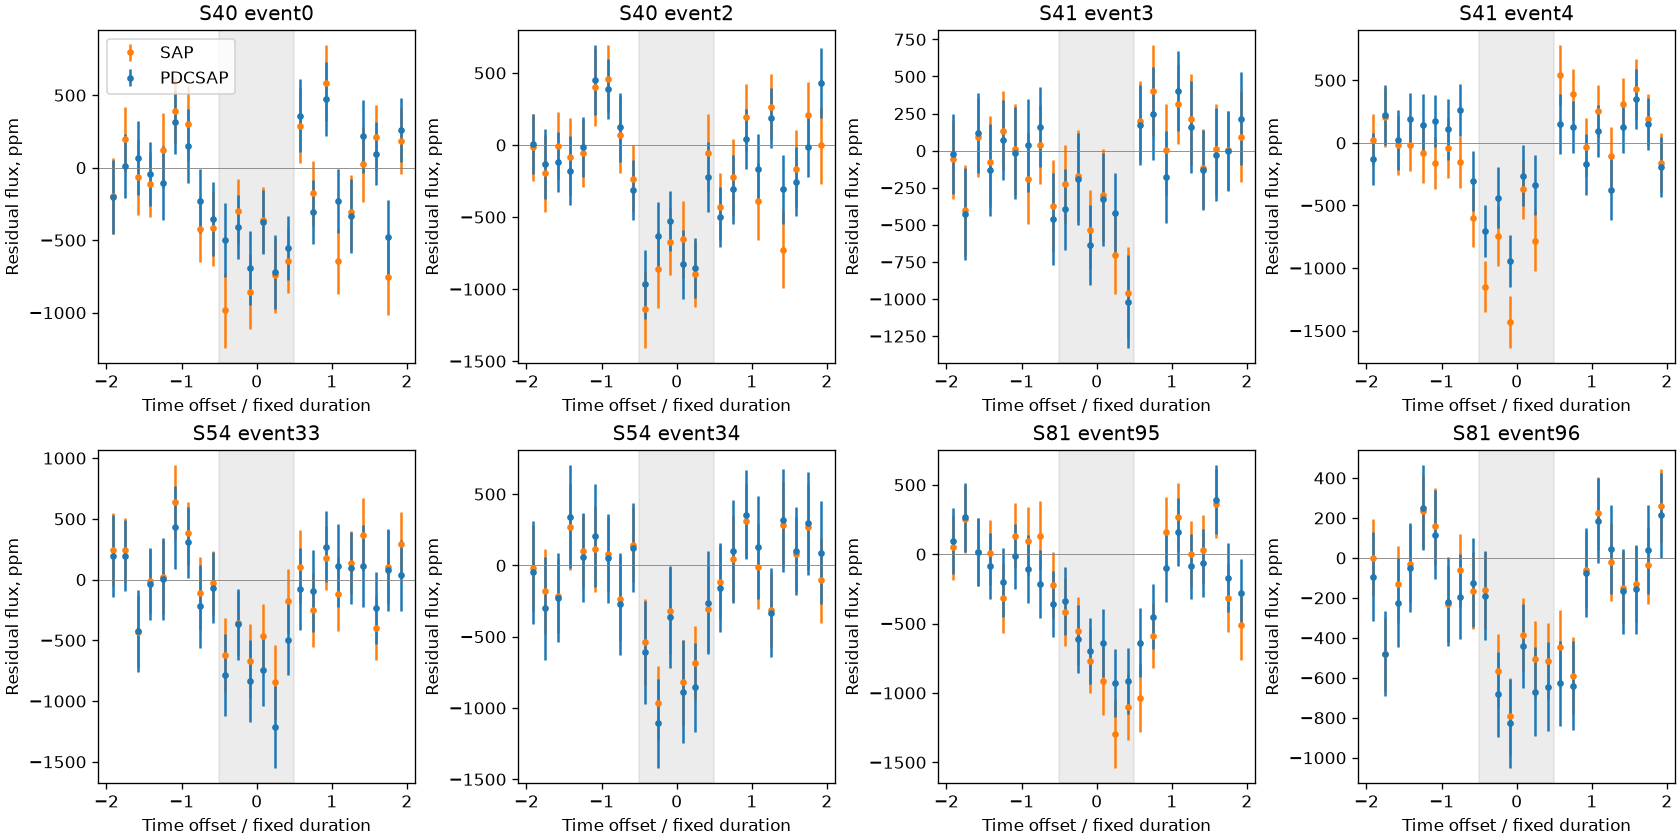
\includegraphics[width=0.98\linewidth]{figures/402-events.png}
\caption{All eight usable TIC 402358350 events, illustrated with the
linear-$3D$ baseline specified in the method matrix. SAP and PDCSAP retain
positive dips and share photons. The protected event intervals and local
baselines test whether additional global smoothing created the feature;
they do not establish the host. Errors follow the conditional measurement
model and do not include all timing or instrumental uncertainty.}
\label{fig:402events}
\end{figure}

\begin{figure}[tbp]
\centering
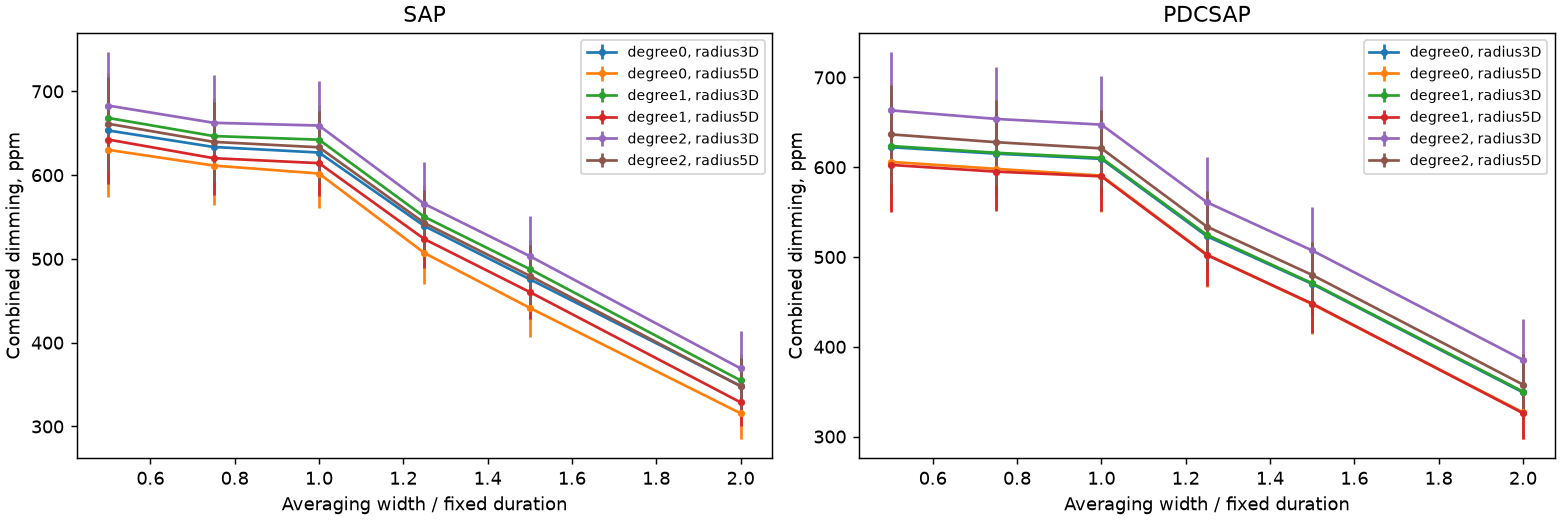
\includegraphics[width=0.96\linewidth]{figures/402-widths.png}
\caption{TIC 402358350's retained averaging-width and baseline matrix.
Central depths are approximately stable between widths $0.5D$ and $D$,
and decrease as wider windows include the shoulders. This supports
localization in time; the displayed widths are fixed diagnostic choices,
not a fitted transit-duration posterior. Rows and columns reuse the same
events and are not independent trials.}
\label{fig:402widths}
\end{figure}

The width tests show a localized depression rather than a uniformly broad
low state (Figure~\ref{fig:402widths}). Adverse controls remain material:
one matched SAP offset window is deeper than its associated event under
five of six baselines, and a sector-54 event has no matched controls.
Time-averaging inflation expands combined errors to 41--93 ppm, depending
on baseline; linear-$3D$ results change only to $642\pm43$ and
$610\pm44$ ppm. Scalar inflation is a sensitivity diagnostic rather than
a full noise likelihood.

The nearby published pulsator TIC 402358249 has dominant frequency
0.9517724 d$^{-1}$ (period 1.050671358 d). Adding sine and cosine nuisance
terms at this fixed frequency leaves SAP depths near 578 ppm and PDCSAP
depths near 610--621 ppm. This rules out only that simple sinusoidal model
as a complete explanation. Conversely, deterministic 1000-ppm sinusoidal
injections into the archived products can shift a sector's box depth by
up to 1209 ppm after sampling and flattening
(Figure~\ref{fig:pulsator}). Smooth variability can therefore couple
strongly into these measurements; the experiment neither bounds the real
contamination nor reruns the upstream telescope reduction.

\begin{figure}[tbp]
\centering
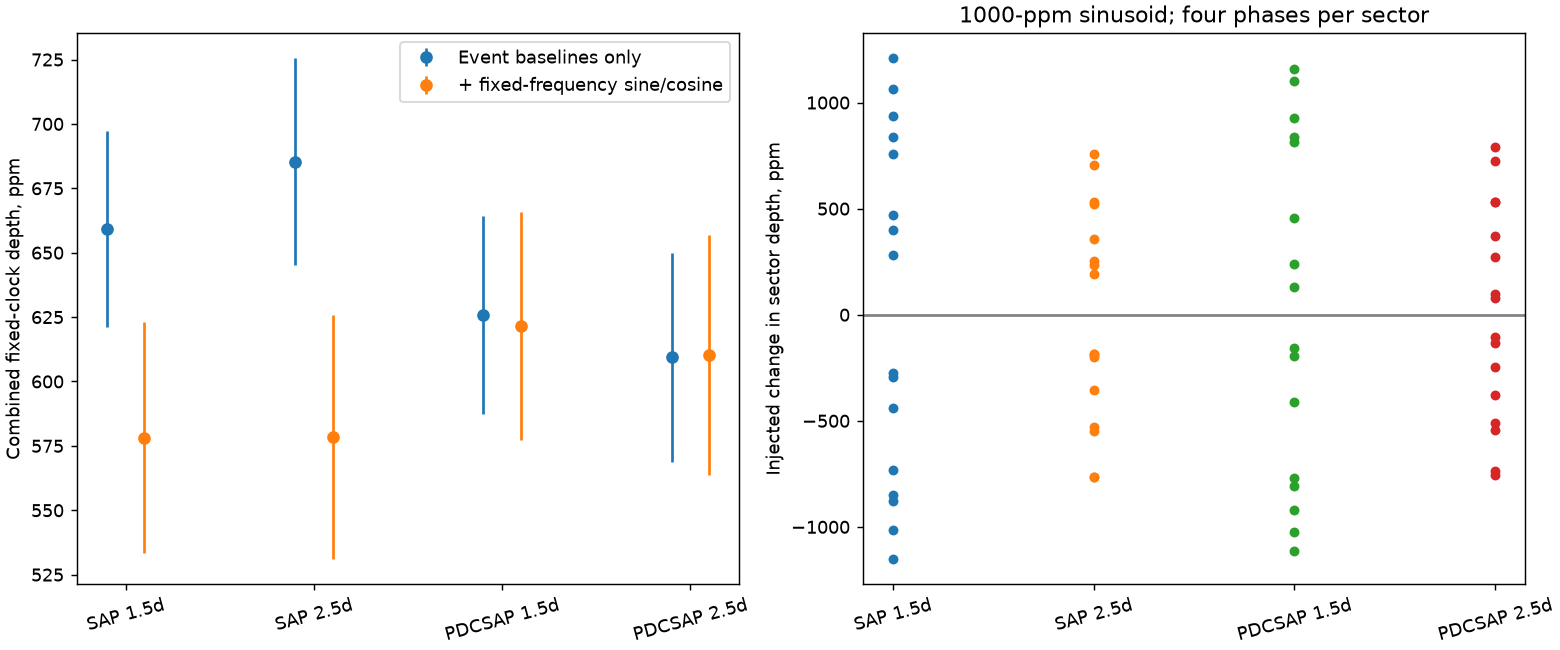
\includegraphics[width=0.96\linewidth]{figures/pulsator-tests.png}
\caption{TIC 402358350's fixed-frequency pulsation nuisance fits and
deterministic sinusoid-transfer tests. The nuisance sinusoid does not
absorb the recurring dip, while the injection response demonstrates
substantial sampling and preprocessing sensitivity. These are
retrospective tests of already inspected products, not independent
observations, an astrophysical contamination model, or a false-alarm
calibration.}
\label{fig:pulsator}
\end{figure}

\section{Source attribution and competing stellar hosts}
\label{sec:host}

Repeatable dimming and identification of its host are separate requirements.
For TIC 80387959, stacked image models prefer the target in sectors 36,
37, and 100, TIC 80387965 in sector 63, and TIC 80387961 in sector 90.
Every sector changes its preferred host under at least one event omission
(Figure~\ref{fig:hostinstability}). For TIC 402358350, the discovery
sectors disagree, while later whole-stamp fits favor the target region
with substantial structured residuals and sensitivity to the fitted image
region. A known shallow planet, Kepler-93 b, is incorrectly assigned a
neighbor preference by this same procedure in one tested sector.
Consequently model rankings, even stable ones, are not calibrated host
probabilities or sufficient planet vetoes.

\begin{figure}[tbp]
\centering
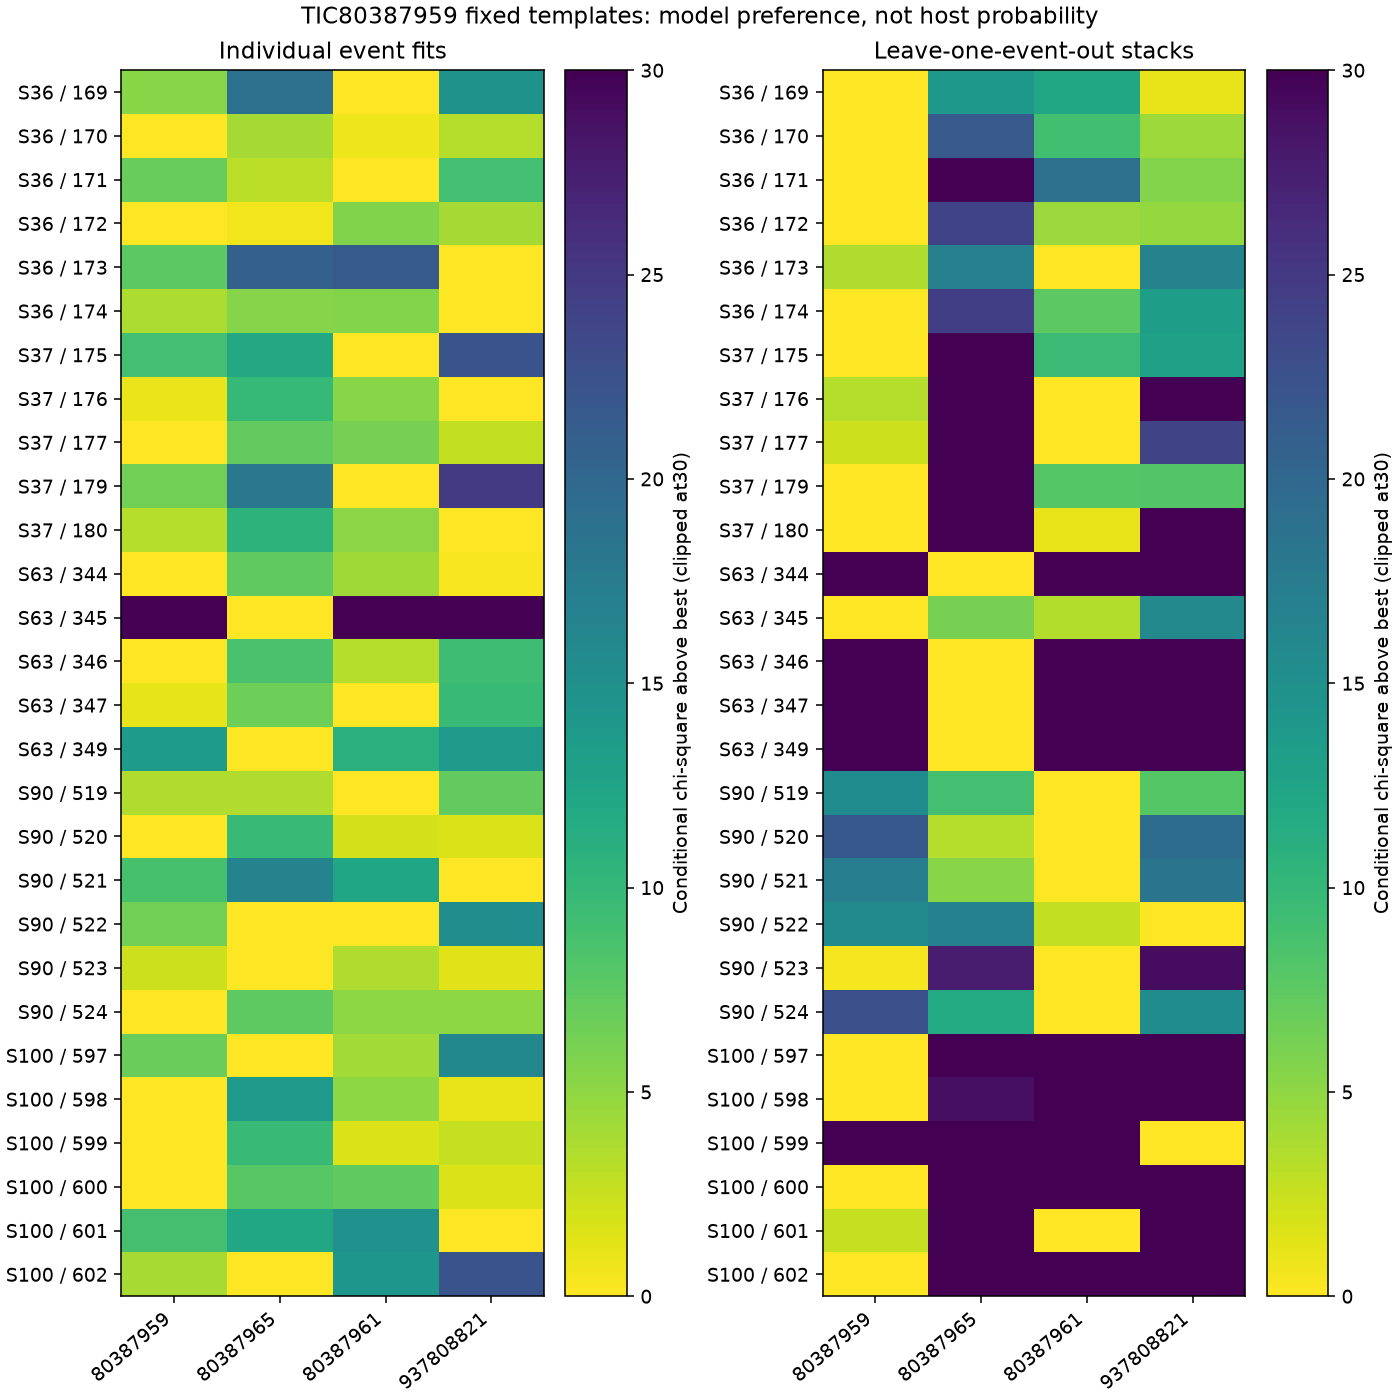
\includegraphics[width=0.96\linewidth]{figures/host-instability.png}
\caption{Event-level and omission sensitivity of TIC 80387959's source
rankings. Different sectors and subsets prefer different stars.
Overlapping omissions are correlated diagnostics. Inadequate image
residuals and a failed known-host control prevent interpreting the
chi-square rankings as probabilities or selecting target-favoring subsets
as definitive source attribution.}
\label{fig:hostinstability}
\end{figure}

The aperture-light budget supplies a complementary constraint
\cite{giacalone2022}. If a neighbor contributes a fraction $f$ of the
aperture light, its intrinsic eclipse must have depth $e=d/f$ to produce
an observed SAP decrement $d$. Under equal target/neighbor throughput,
TIC 80387965, 13.76 arcsec away, needs approximately 1.41--1.72\%
eclipses; TIC 80387961, 7.54 arcsec away, needs 24.19--29.47\%.
For TIC 402358350, TIC 1918682563 at 10.12 arcsec needs
24.76--28.86\%. These are conditional requirements, not observed
eclipses. Some fainter competitors exceed 100\% under nominal assumptions,
but uncertain response, catalog identity, magnitude, and depth reopen them
in the declared sensitivity tests (Figure~\ref{fig:eclipsebudget}). No
listed close competitor is safely excluded, and unresolved companions
are unconstrained by this resolved-source budget.

\begin{figure}[tbp]
\centering
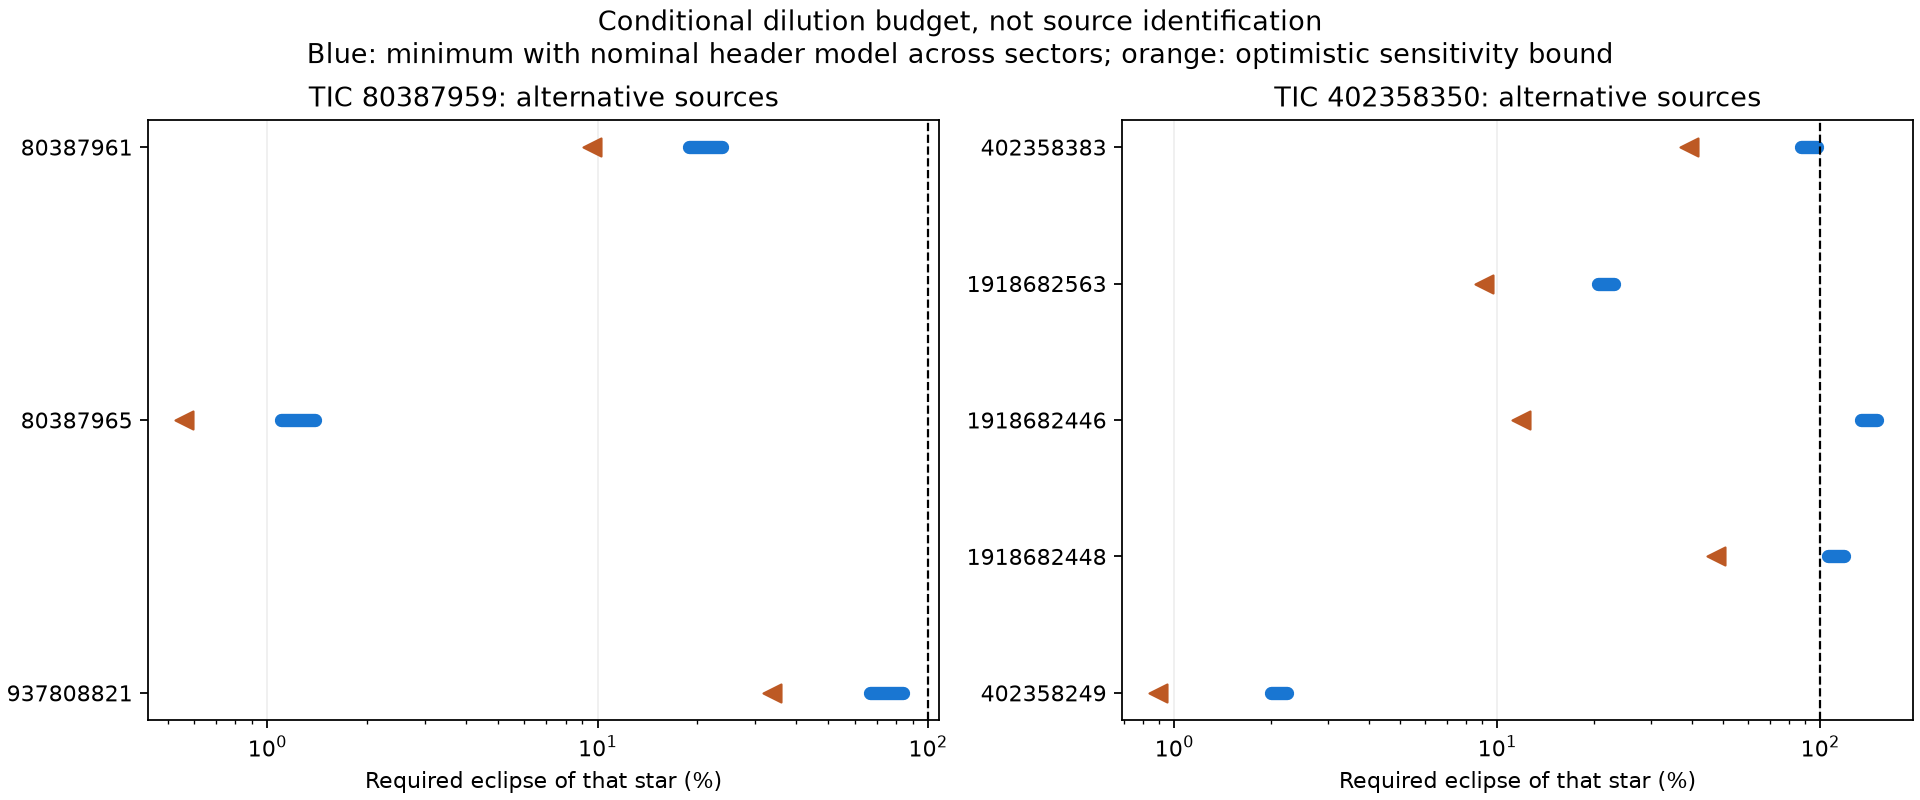
\includegraphics[width=0.97\linewidth]{figures/host-eclipses.png}
\caption{Conditional intrinsic eclipses required on nearby sources.
Requirements use native SAP decrements and alternative aperture-response
assumptions. Pipeline crowding and captured-flux estimates are models,
not independent response measurements. The optimistic cases are declared
stress tests rather than confidence limits. A nominal requirement above
100\% does not exclude a source whose catalog or throughput model is
uncertain.}
\label{fig:eclipsebudget}
\end{figure}

Resolved archival photometry has not closed this gap. For TIC 80387968,
35.34 arcsec from TIC 80387959, 43 quality-selected SkyMapper measurements
include two differently colored samples during one predicted event, with
no dimming. They disfavor a particular same-depth, flat-bottom eclipse at
those instants, but fail the predeclared two-event exclusion gate.
Color, eclipse shape, and calibration remain limitations. Around
TIC 402358350, four ZTF streams for TIC 1918682563 retain 288 accepted
measurements with large scatter; all 48 fixed-clock comparisons are
inconclusive. A separate six-stream test of TIC 74037550 retains 545
measurements and all 72 comparisons are inconclusive. Sparse sampling and
propagated timing uncertainty prevent eclipse exclusions, even where
nominal precision would otherwise appear sufficient.

\section{Conditional astrophysical scenario calculations}
\label{sec:models}

We used TRICERATOPS 1.1.0 \cite{giacalone2021} as an exploratory comparison
of astrophysical scenarios, applying it to one already examined sector per
target: sector 36 for TIC 80387959 and sector 54 for TIC 402358350.
The native SAP inputs remove previously fitted event baselines, retaining
482 samples from six events and 230 samples from two events, respectively.
The calculations use the diluted-flux convention and explicit exposure
integration. Baseline covariance is not marginalized, stellar parameters
are held fixed, and a nominal Gaussian aperture response controls nearby
host eligibility. Verified exact catalog duplicates were removed while
preserving the superseded inputs and calculations.

All 17 bounded runs and three provenance replays were completed. The
nominal set contains three 100,000-draw seeds and one million-draw seed
per target; the remaining runs test noise sensitivity and diagnostic
controls. Table~\ref{tab:triceratops} gives the million-draw values.
The original requirement of three independent million-draw calculations
per target was not met, so convergence is unestablished. Three smaller
seeds span 92.2334--92.7963\% and 97.3632--97.8000\% in target-primary
weight; these ranges measure numerical scatter rather than physical
uncertainty (Figure~\ref{fig:triceratops}).

\begin{table}[tbp]
\centering
\caption{Single-seed, million-draw TRICERATOPS scenario weights.
These are conditional on the supplied single-sector data and modeled
scenarios; neither target passes the joint numerical validation thresholds.}
\label{tab:triceratops}
\begin{tabular}{lrrr}
\toprule
TIC & Target-primary planet weight & FPP & NFPP \\
\midrule
80387959  & 92.4284\% & 7.5716\% & 4.2862\% \\
402358350 & 97.6834\% & 2.3166\% & 0.3959\% \\
\bottomrule
\end{tabular}
\end{table}

\begin{figure}[tbp]
\centering
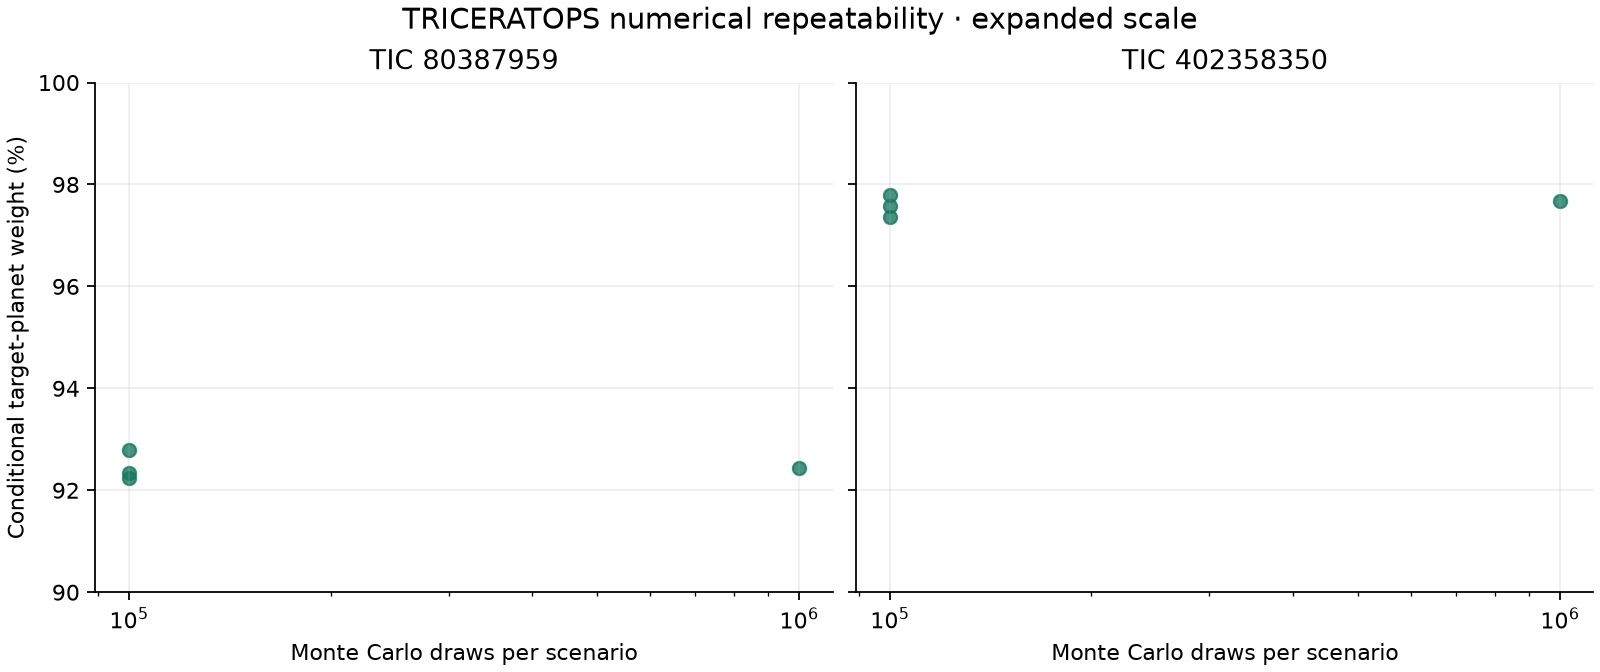
\includegraphics[width=0.96\linewidth]{figures/triceratops-convergence.png}
\caption{Adopted nominal TRICERATOPS runs at two draw counts.
Repeated smaller calculations test Monte Carlo sensitivity, but one
million-draw seed per target leaves the original convergence criterion
unmet. The scenario weights exclude general artifacts and stellar
variability, and do not quantify discovery reliability. The two targets
also retain different observational timing and attribution limitations.}
\label{fig:triceratops}
\end{figure}

Here $1-\mathrm{FPP}$ sums planet scenarios around the target primary,
including the package's dilution alternatives. FPP includes some planets
on other stars; NFPP includes all resolved-neighbor scenarios, including
neighboring planets. Neither candidate meets both published numerical
criteria, $\mathrm{FPP}<0.015$ and $\mathrm{NFPP}<0.001$; both also fail
the nearby-source threshold for the method's less restrictive
``likely planet'' category. These thresholds do not independently transfer
the calibration of the published workflow to the present exploratory inputs.

The omitted-model problem is visible in controls. Setting the flux
identically to unity still yields target-primary planet weights of
44.15\% and 23.38\%; inverted signals yield 41.99\% and 15.91\%.
These tests retain the supplied clock and observed-depth host eligibility,
so they are computational diagnostics, not false-alarm experiments.
Doubling the scalar noise changes nominal weights to 91.98\% and 93.74\%.
The restricted Kepler-93 b control returns 82.88\% and fails the validation
thresholds despite that planet's independent establishment. The scenario
family lacks general instrumental and stochastic stellar-variability
alternatives and normalizes its weights even for unconvincing inputs.
Accordingly these percentages do not measure the probability of a real
planet or a new discovery. TIC 402358350's larger weight does not repair
its timing failure or make its overall evidence stronger than that for
TIC 80387959.
